\chapter{基于STRIDE对车载IVI系统的威胁建模}
\label{ch3}
本章首先介绍了威胁建模步骤,对威胁建模的步骤进行了详尽阐述
分析,最后基于STRIDE威胁模型对一个车载系统进行实例威胁分析和风险评估。
\section{威胁建模步骤}
要进行有效的威胁建模,首先需要以下利益相关者的意见:
  \begin{itemize}
    \item 提供应用程序的业务影响的业务利益相关者。
    \item 架构师提供应用生态系统的概述。
    \item 用于特定代码输入的程序员,例如使用的框架、编码指南等。
    \item DevOps提供服务器和网络配置的详细信息。
    \item 专家学者在关键参数上的影响因子
  \end{itemize}
  其次是威胁建模的具体步骤,图3.1是威胁建模的步骤图:
  \begin{itemize}
    \item 设计:明确系统的所有要求,并创建数据流关系图。
    \item 中断: 将威胁建模框架应用到数据流关系图,并查找潜在的安全问题。
    \item 修复: 确定如何正确组合安全控制来解决每个问题。
    \item 验证: 验证是否满足了要求、找到了问题并实现了安全控制。
  \end{itemize}
  \begin{figure}
    \centering
    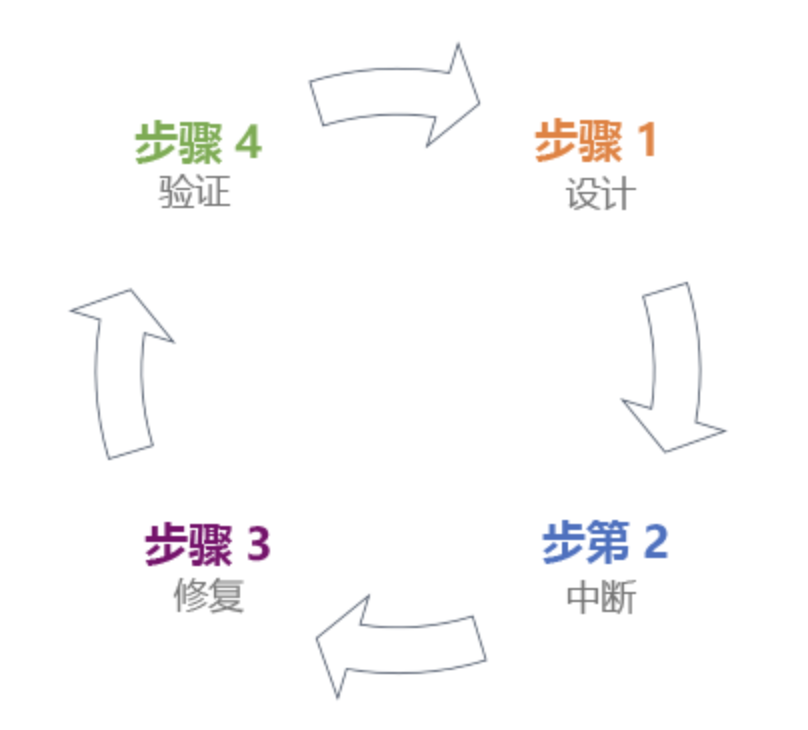
\includegraphics[scale=0.6]{resources/img/i4.png}
    \caption{威胁建模步骤}
  \end{figure}

\subsection{设计}
设计阶段是进行威胁建模活动的基础。 你需要尽可能多地收集关于你所构建的内容及所用资源的数据。
清楚地了解系统的工作原理,列出系统使用的每个服务,枚举有关环境和默认安全配置的所有假设,使用正确的上下文深度级别创建数据流关系图。
尽可能多地提出有关系统的问题。 可以考虑以下问题:
保护数据免受未经授权的披露的机密性。
防止未经授权的信息更改的完整性。
即使系统受到攻击也能提供所需的服务。
系统如何处理密钥、证书和凭据?
需要保护哪些商业秘密和知识产权?
想在威胁建模上花费多少时间和金钱?
\newline
在设计阶段"可视化"是非常重要的步骤.对整个应用程序的清晰记录的概述将大大简化流程。这包括记下用例、数据流、数据模式和部署图。您可以构建两种类型的可视化。
数据流图:它描述了数据是如何设计为在您的系统中移动的。它显示了操作级别,并清楚地显示了数据进入和退出每个组件的位置、数据存储、流程、交互和信任边界。 
流程图:它描述了用户如何在各种用例中交互和移动。它处于应用程序级别。DFD 专注于系统内部的工作方式,而 PFD 则专注于用户和第三方与系统的交互。您可以选择其中之一或同时使用两者。
这里介绍下创建数据流关系图: 数据流关系图是系统的图形表示形式,应指定每个元素及其交互和上下文。
数据流关系图显示了给定系统中的数据流。 它通常以用户或数据存储的请求开始,以数据存储或 Analytics Services 结束。 数据流关系图使用不同的形状来指示它们所表示的元素。
如元素:过程一般用圆形来表示,其定义:接收、修改输入或将输入重定向到输出的任务,如 Web 服务。
外部实体用矩形来表示,其定义:直接控制之外的任务、实体或数据存储,如用户和第三方 API。
数据存储一般用形如"二"汉字来表示,其定义:永久和临时数据存储,如 Web 缓存和 Azure 托管数据库。
数据流关系图应当包含:正在构建的系统类型和安全团队所需的上下文。	

\subsection{中断}
在中断阶段,需使用数据流关系图查找针对系统的潜在威胁。 此过程使用威胁建模框架,以帮助你查找最常见的威胁和防范威胁的方法。
选择以“保护系统”或“了解攻击者”为核心的方法, 如使用微软的STIRIDE威胁模型识别常见威胁。
选择重点领域和相关框架,以系统地识别系统中的潜在威胁。

\subsection{修复}

在修复阶段,需要决定如何处理所有威胁。 比如每个STRIDE威胁都对应到一项或多项安全控制,这些控制措施提供不同的功能和类型供你选择。
并且获得与每个资产及其操作相关的威胁的主列表或库以及可能的攻击者配置文件列表。
具体来讲:该阶段目标如下:
\begin{itemize}
    \item 根据优先级框架或安全 bug 栏衡量每个威胁的优先级
    \item 将每个威胁作为任务或工作项进行跟踪
    \item 生成对应于 STRIDE 威胁的安全控制建议
    \item 选择一项或多项安全控制类型和功能来应对每个威胁
    \item 解决任务
  \end{itemize}

\subsection{验证}

验证阶段是威胁建模过程的最后一步,通常发生在部署系统之前。 它涉及到确保满足要求、验证假设以及准备好安全控制。
确认系统满足所有新旧安全要求,配置云提供商、操作系统和组件以满足安全要求,确保使用正确的安全控制解决所有问题,在部署前对系统进行手动和自动验证。
在验证期间,需要我们检查是否所有漏洞都已得到解决。并自问以下问题:所有的威胁都被缓解了吗?是否清楚地记录了剩余风险?
完成此操作后,需要决定管理已识别威胁的后续步骤,并决定下一次威胁建模迭代的时间。
威胁建模不是一次性活动。它需要在预定的时间间隔或在应用程序开发的特定里程碑期间重复。


\section{STRIDE威胁建模实例}
由于在第四章提出的威胁建模风险评估模型是基于传统的STRIDE模型来的, 因此本节将通过传统的STRIDE模型对智能网联汽车车载娱乐系统IVI进行威胁建模,并以此为例对此进行风险评估
为后续的新型风险评估模型进行前置理论基础。

\subsection{车载娱乐STRIDE威胁模型}
威胁识别是对信息系统划分的各个数据流构建STRIDE
威胁建模,分析每个数据流及其关联的资产是否容易受到S、 T、R、I、D以及E类威胁的攻击,识别并记录这些威胁。该IVI系统数据流的STRIDE威胁模型如图3.2所示。
\begin{figure}
  \centering
  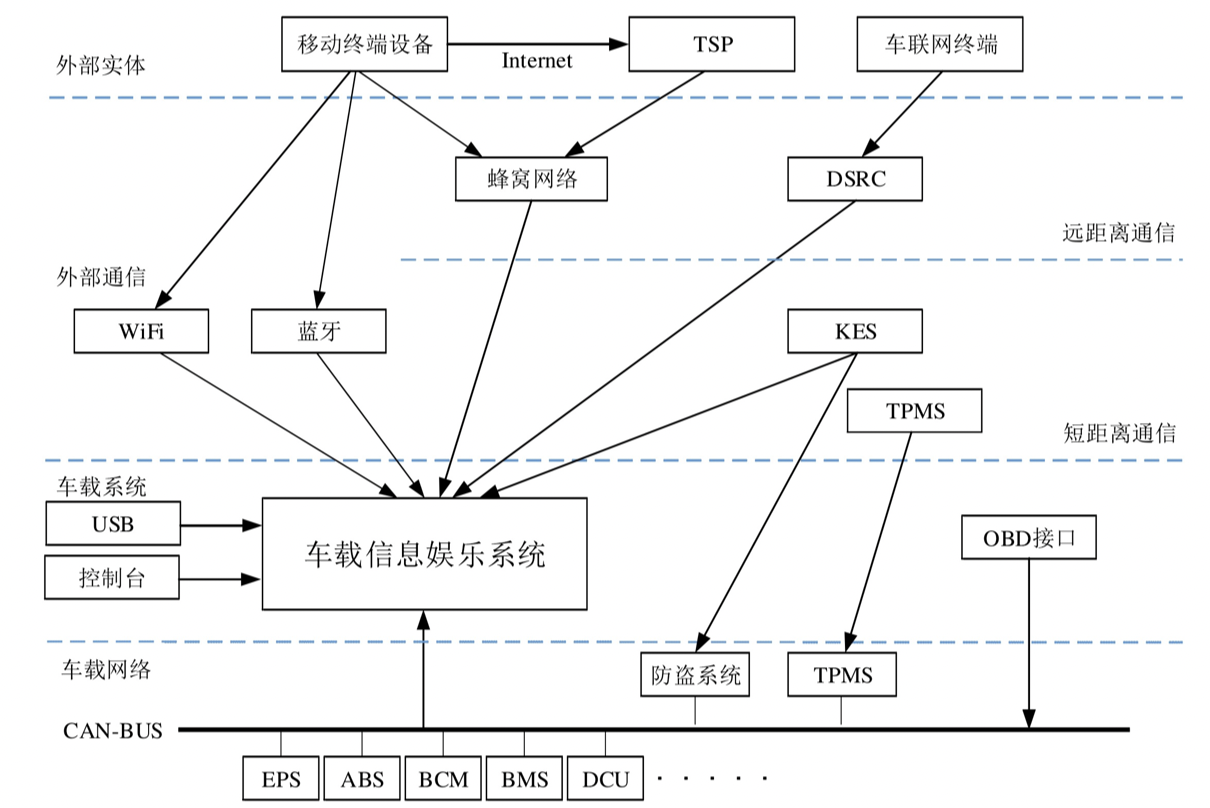
\includegraphics[scale=0.6]{resources/img/i33.png}
  \caption{车载娱乐IVI系统安全威胁建模图}
\end{figure}
\subsection{DF数据流威胁描述}
这里我们对三个外部元素:WIFI, USB, GPS 进行威胁评级描述分析
并把它们的数据流分别称为: DF1, DF2, DF3。
\newline
(1)DF1 WIFI与智能网联汽车IVI车载娱乐系统交互
该数据流可能面临的威胁有:攻击者通过劫持路由器伪装Wi-Fi信号, 窃听用户传输信息\cite{berghel2005wifi}

(2)DF2 USB与智能网联汽车IVI车载娱乐系统交互
该数据流可能面临的威胁有:通过USB设备的固件进行重新编程,来执行恶意行为,比如恶意文件下载、数据泄露等\cite{nissim2017usb}。

(3)DF2 GPS与智能网联汽车IVI车载娱乐系统交互
该数据流可能面临的威胁有:通过对搭载GPS传感器的车载信号接收器发送虚假信号, 从而误导汽车导航定位等\cite{alamleh2020cheat}。
\subsection{威胁评级}
我们通过STRIDE的五个属性即第二章提到的威胁评级给这实体威胁进行评分:
Wi-Fi 信号,潜在损失 D,可获得很多信息,所以打分为 3;重现性 R,Wi-Fi 可重现
性较强,评分为 3;可利用性,路由器的设置也极为简单,评分为 4;受影响用户 A 影响的一般是普通用户,评分为 2;
可发现性,较为容易发现,评分为 2。再根据评级公式,可得出最后的威胁评级 Rank = (3 + 2 + 4 + 2 + 2) ÷ 2 = 6.5。
USB,潜在损失 D,可获得很多信息,所以打分为 3;重现性 R, 可重现
性较强,评分为 3;可利用性,由于要进入车体连接USB较难实现,可利用性低评分为 1;受影响用户 A 影响的一般是普通用户,评分为 2;
可发现性,较为容易发现,评分为 2。再根据评级公式,可得出最后的威胁评级 Rank = (3 + 2 + 4 + 1 + 2) ÷ 2 = 6。
GPS,潜在损失 D,可获得很多信息,所以打分为 3;重现性 R, 可重现
性较低,评分为 1;可利用性,由于要通过伪造信号基站成本较高,可利用性低评分为 1;受影响用户 A 影响的一般是普通用户,评分为 2;
可发现性,较难发现,评分为 3。再根据评级公式,可得出最后的威胁评级 Rank = (3 + 1 + 1 + 2 + 3) ÷ 2 = 5。
如表3.1我们给出了GPS的威胁列表
\begin{table}
  \caption{GPS威胁列表}
\begin{center}
    \begin{tabular}{|l|l}
      \hline 威胁编号 & A2 \\
      \hline 元素实例 & GPS \\
      \hline 威胁类别 & Spoofing \\
      \hline 威胁描述 & 伪装假GPS信号 影响用户GPS功能 \\
      \hline 威胁评级 & 5 \\
      \hline 消减威胁 & 升级GPS固件加固GPS信号和其他辅助导航软件 \\
      \hline
      \end{tabular}
  \end{center}
\end{table}


\section{本章小结}
本章首先详细阐述威胁建模方法论原理和步骤,梳理威胁的存在和建模流程。
最后还通过应用STRIDE威胁模型进行实例威胁建模,对智能网联汽车IVI系统进行了威胁分析和风险评估,
为第四章的全新SATT威胁建模方法提供理论基础,为第五章的实际商用攻击实例提供实例参考。